\subsection{Reconstruction level UE versus jet observables}
The reconstructed level underlying event measurement is shown via the mean transverse energy density of full calorimeter topoclusters as a function of leading jet $\pT$ in Figure~\ref{fig:reco_ue_pt}. 
Fairly good agreement is seen between data and monte carlo for these uncorrected distributions prior to unfolding.
\begin{figure}
    \centering
    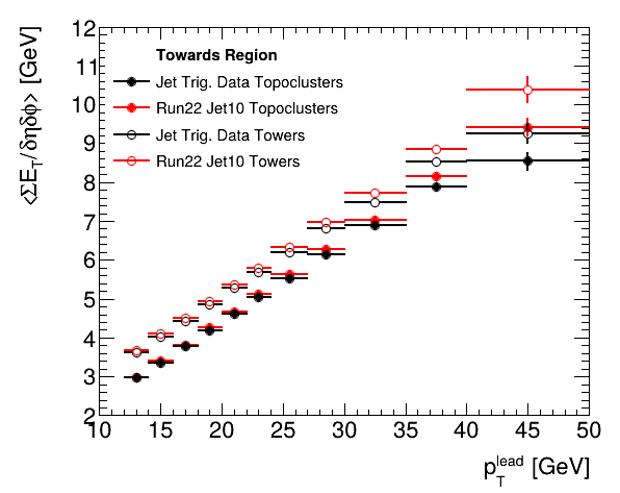
\includegraphics[width=0.48\linewidth]{Figures/unfolding/reco_ue_pt_towards.png}
    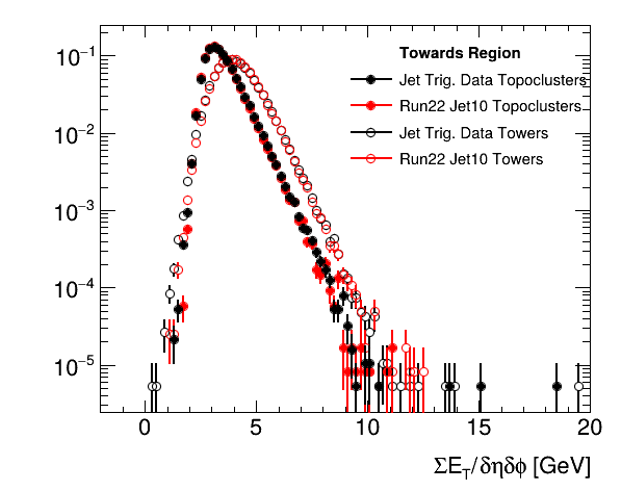
\includegraphics[width=0.48\linewidth]{Figures/topocluster_noise/towards_ET.png}
    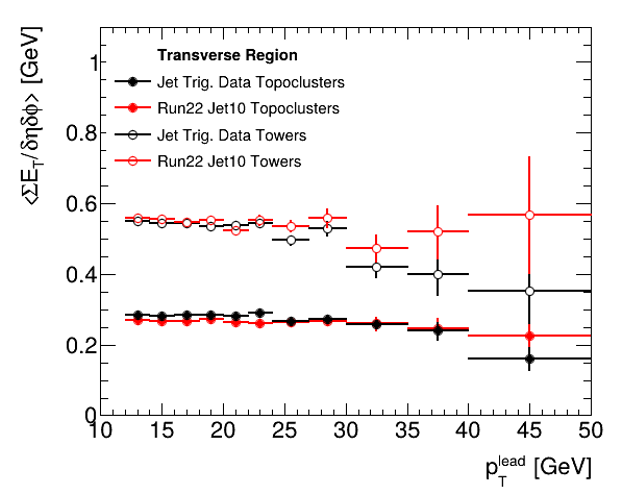
\includegraphics[width=0.48\linewidth]{Figures/unfolding/reco_ue_pt_transverse.png}
    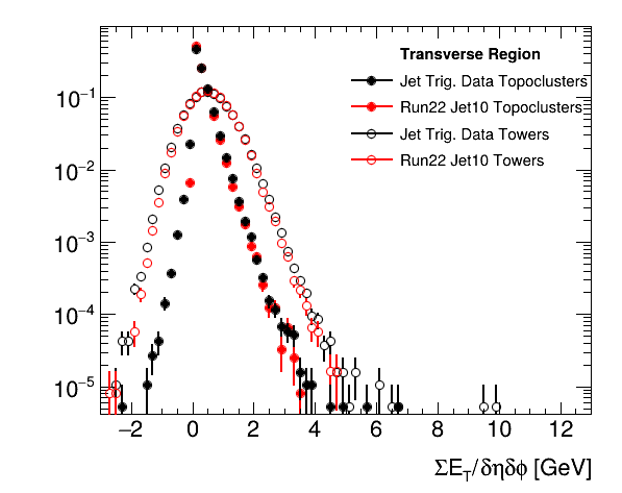
\includegraphics[width=0.48\linewidth]{Figures/topocluster_noise/transverse_ET.png}
    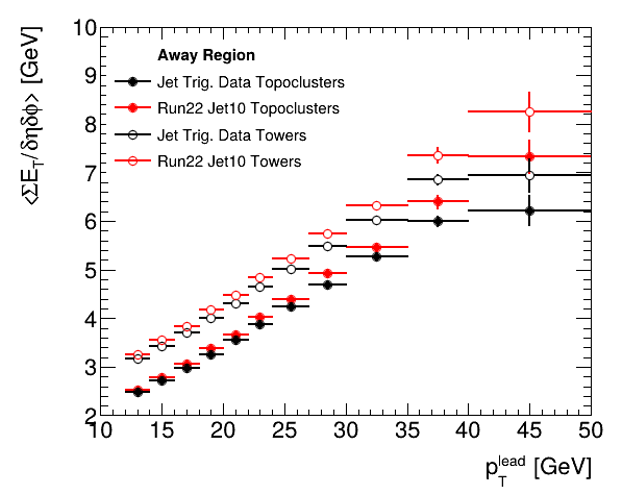
\includegraphics[width=0.48\linewidth]{Figures/unfolding/reco_ue_pt_away.png}
    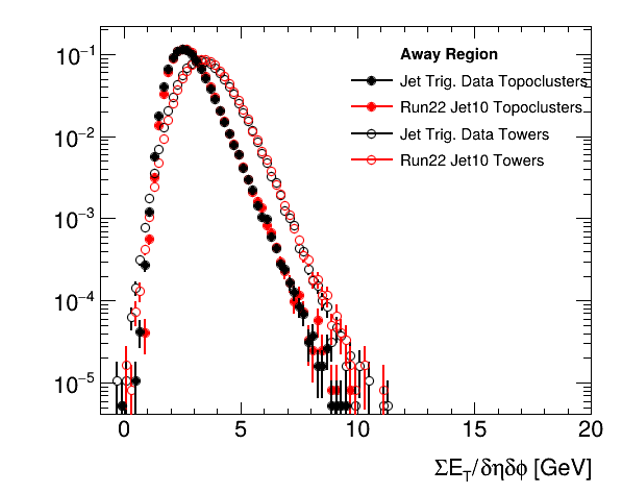
\includegraphics[width=0.48\linewidth]{Figures/topocluster_noise/away_ET.png}
    \caption{Comparison of reconstructed level mean topocluster (tower) transverse energy versus leading jet $p_{T}$ in dijet events (left) and reconstructed level topocluster (tower) transverse energy distributions (right) for towards (top), transverse (center) and away (bottom) jet regions.}
    \label{fig:reco_ue_pt}
\end{figure}

\subsection{Monte Carlo Sample Combination}
\label{sec:mc_samples}

The full set of triggered MC samples used in this analysis need to be weighted by cross section weights before combined to create a smooth jet spectra for comparison to data and use in unfolding procedure.
As a validation step on the cross section weights determined from the pythia cross section values and filtering weights for each triggered MC sample, the truth and reconstructed leading jet spectra are shown in Figure~\ref{fig:mc_sample_distributions}. Figure~\ref{fig:mc_sample_distributions} also shows the contributions to the transverse region $E_{T}$ measurement from each of the triggered MC samples and from these plots we can see strong overlap in the $E_{T}$ spectra for different jet triggered samples as well as the extent to which the $E_{T}$ distribution extends out which helps to determine what a reasonable high $E_{T}$ threshold is for our response matrix and data histograms.

\begin{figure}
    \centering
    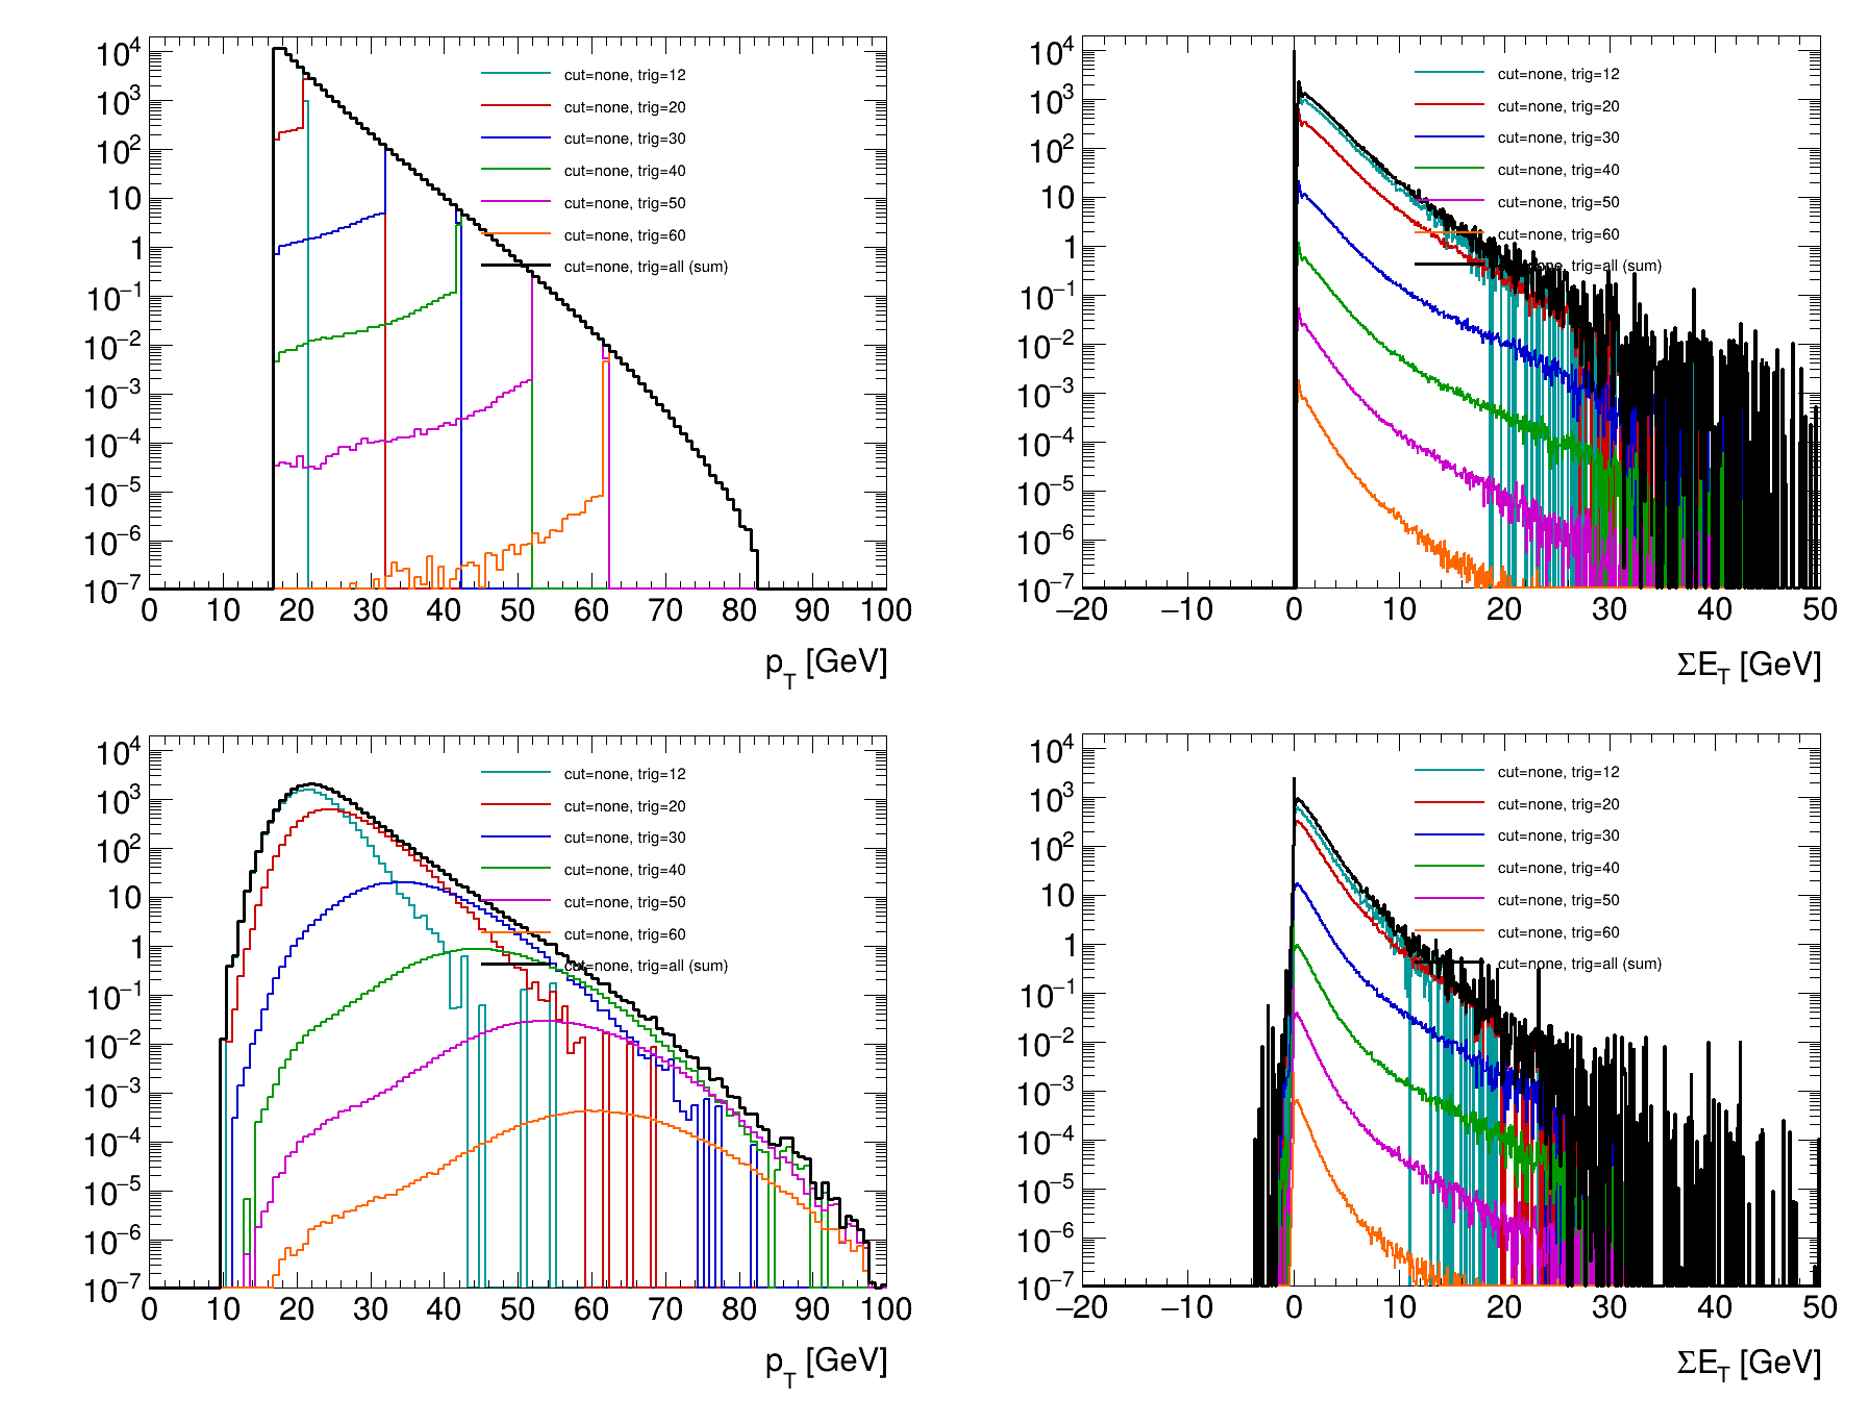
\includegraphics[width=\linewidth]{Figures/unfolding/MC_sample_distributions_inclusive.png}
    \caption{Plots of truth leading jet $p_{T}$ spectra (top left), reconstruction level calibrated leading jet $p_{T}$ spectra (top right), truth transverse region $E_{T}$ (bottom left) and reconstruction level transverse region $E_{T}$ (bottom right) for each MC triggered sample and the full MC distribution with cross section weighting.}
    \label{fig:mc_sample_distributions}
\end{figure}

\subsection{Monte Carlo Vertex Reweighting}
\label{sec:mc_vertex_reweighting}

Monte Carlo events are reweighted to match the $z_{\mathrm{vtx}}$ distribution observed in data. 
Figure~\ref{fig:mc_vertex_reweighting} shows the $z_{\mathrm{vtx}}$ distribution for data and Monte Carlo events.
\begin{figure}
    \centering
    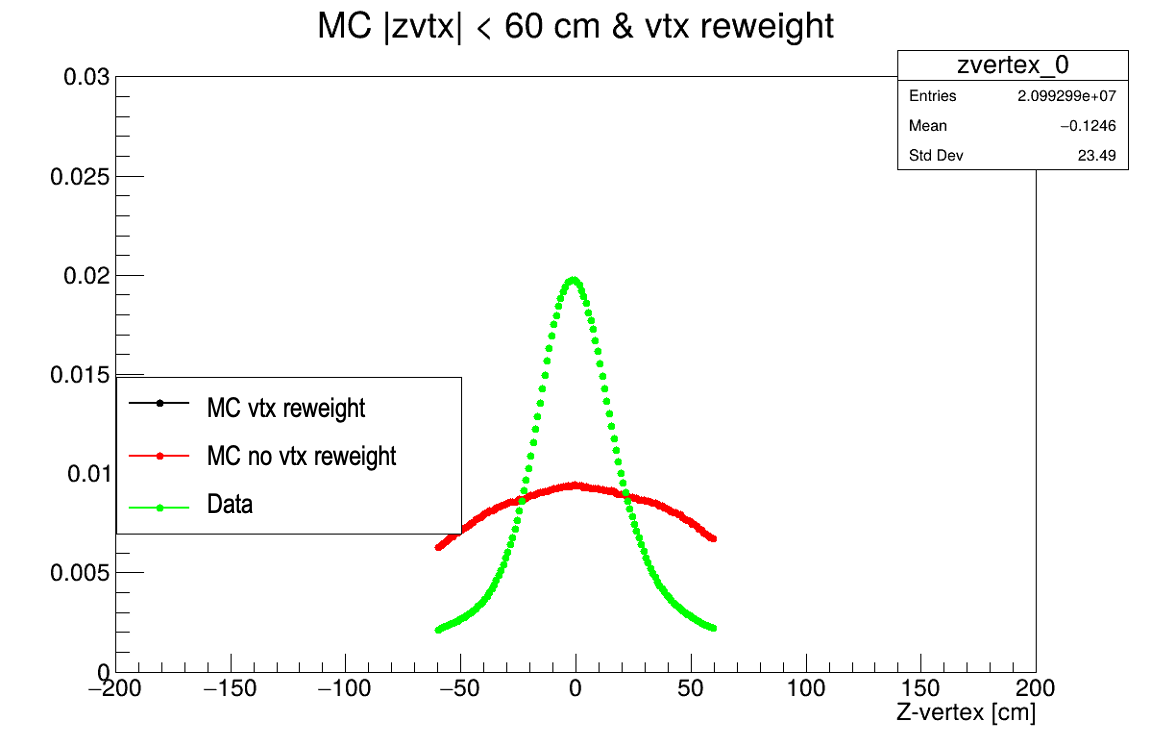
\includegraphics[width=0.7\linewidth]{Figures/unfolding/mc_vertex_reweight_w_data.png}
    \caption{Comparison of $z_{\mathrm{vtx}}$ distribution for data (green) and both unweighted (red)and weighted (black) MC events.}
    \label{fig:mc_vertex_reweighting}
\end{figure}

The effect of this reweighting is evaluated at both truth and reconstructed levels. 
Figure~\ref{fig:vertex_reweighting} compares truth leading jet $p_{T}$, truth transverse region $\Sigma E_{T}$, calibrated leading jet $p_{T}$, and reconstruction level transverse region $\Sigma E_{T}$ distributions before and after vertex reweighting.
No significant modification for the truth or reco level jet and $E_{T}$ distributions is observed. 

\begin{figure}
    \centering
    \begin{subfigure}[t]{0.48\linewidth}
        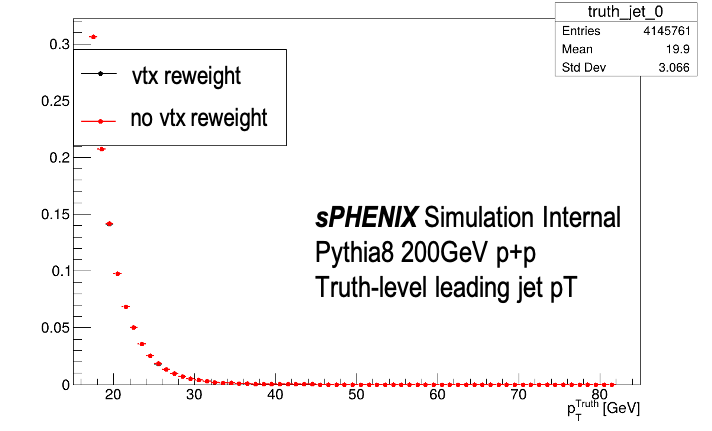
\includegraphics[width=\linewidth]{Figures/unfolding/mc_vertex_reweight_truthjet.png}
        \caption{Truth jet $p_{T}$}
    \end{subfigure}
    \hfill
    \begin{subfigure}[t]{0.48\linewidth}
        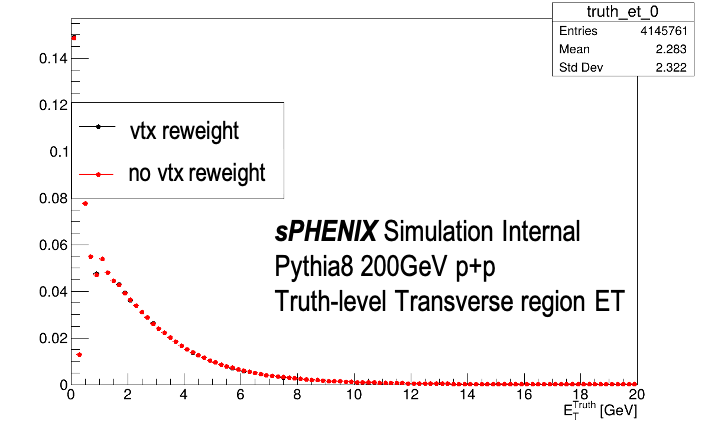
\includegraphics[width=\linewidth]{Figures/unfolding/mc_vertex_reweight_truthet.png}
        \caption{Truth $E_{T}$}
    \end{subfigure}
    \vspace{0.4em}
    \begin{subfigure}[t]{0.48\linewidth}
        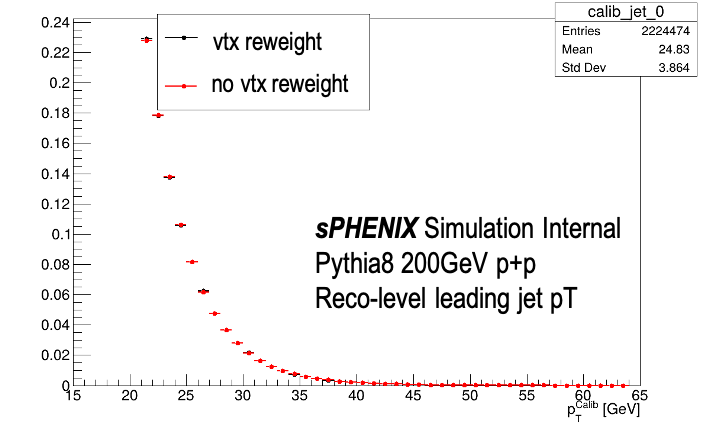
\includegraphics[width=\linewidth]{Figures/unfolding/mc_vertex_reweight_calibjet.png}
        \caption{Calibrated jet $p_{T}$}
    \end{subfigure}
    \hfill
    \begin{subfigure}[t]{0.48\linewidth}
        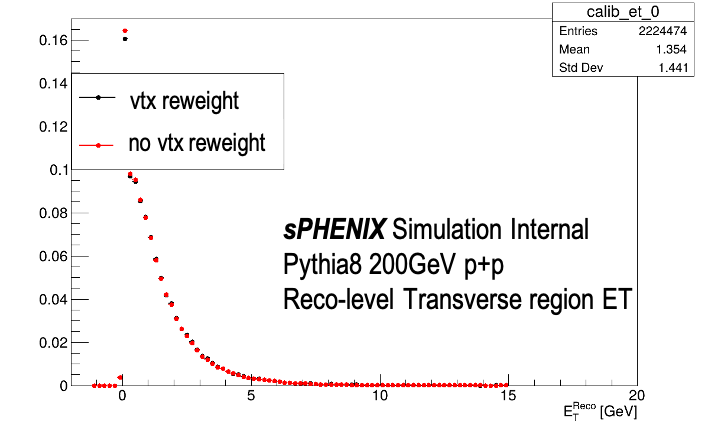
\includegraphics[width=\linewidth]{Figures/unfolding/mc_vertex_reweight_recoet.png}
        \caption{Calibrated $E_{T}$}
    \end{subfigure}
    \caption{Distributions before and after MC vertex reweighting at truth and calibrated reconstruction levels.}
    \label{fig:vertex_reweighting}
\end{figure}

\subsection{Unfolding Procedure}
\label{sec:unfolding}

\subsubsection{Simulation Processing for Unfolding Procedure}
The simulation processing module builds the unfolding response matrix from Run-28 jet-triggered samples by applying the same kinematic selections used in the data and outlined in Table~\ref{tab:sim_unfold_processing}. 
Events are required to have a valid vertex ($|z_{\mathrm{vtx}}|<60$ cm) and are weighted by the $z$-vertex reweighting histogram determined from the MC vertex reweighting procedure. 
Events are restricted to a trigger window for the given sample (jet5--jet60) based on their leading truth jet $p_{T}$, truth jets are filtered to enforce $|\eta| \le 0.7$, and reconstructed jets are filtered to remove jets that do not fall fully within the calorimeter detector acceptance (for example part of the jet is clipped at high $\eta$), enforce $|\eta| \le 0.7$, and require positive energy. 
Events with nine or more reconstructed jets above 5~GeV are rejected as bad events.
After filtering, either truth or reconstructed jets must satisfy the minimum good jet multiplicity for jets passing acceptance filters and with $p_{T}> 2$ GeV (1 for inclusive, 2 for dijet). 
For the dijet selection, the leading and subleading jets must satisfy the energy ratio requirement ($E_{\mathrm{sub}}/E_{\mathrm{lead}}>0.3$) and an azimuthal separation cut ($\Delta\phi>\Delta\phi_{\mathrm{min}}$). 
For the inclusive selection, an energy-fraction cut on the leading jet is applied to reject beam background streak events which deposit nearly all of their energy into a single calorimeter layer. 
Reconstructed leading jets are then calibrated using the JES correction function and a JER smearing term of 10.1\% determined from PPG08 studies~\cite{ppg08AN}, and truth and calibrated jets are matched with $\Delta R < 0.75R$. 

The transverse region $E_{T}$ is determined by summming clusters with $\pi/3 < |\Delta\phi| < 2\pi/3$ relative to the leading jet. 
When clusters are used, the transverse $\Sigma E_{T}$ calculated from the sum of cluster transverse energy ($E_{clus}/\cosh(\eta)$). 
Truth $\Sigma E_{T}$ uses final-state particles within $|\eta|<1.1$ and applies the per-particle energy thresholds used for the analysis (0.5~GeV for hadrons and 0.2~GeV for EM particles).

\begin{table}[t]
    \centering
    \small
    \begin{tabular}{ll}
        \hline
        Simulation Selection & Definition \\
        \hline
        Vertex cut & $|z_{\mathrm{vtx}}|<60$ cm \\
        Truth jet lead $p_{T}$ window & jet5--jet60 sample full efficiency ranges \\
        Jet acceptance & $|\eta| \le 0.7$, positive energy, calo-$\eta$ acceptance (reco only) \\
        N$_{jet}$ background cut & reject events with $\ge 9$ jets ($p_{T}\ge 5$ GeV) \\
        Dijet background cut & $E_{\mathrm{sub}}/E_{\mathrm{lead}}>0.3$, $\Delta\phi>\Delta\phi_{\mathrm{min}} = 3\pi /4$ \\
        Inclusive jet background cut & EMCal(10-90\%)/IHCal(0-90\%)/OHCal(10-90\%) lead jet E-fraction cut \\
        Truth and reco jet matching & $\Delta R < 0.75R$ \\
        Truth and reco transverse region & $\pi/3 < |\Delta\phi| < 2\pi/3$ from leading jet $\phi$ \\
        Truth UE particle threshold & $E>0.5$ GeV hadrons, $E>0.2$ GeV EM particles, $|\eta|<1.1$ \\
        Response trimming & trim values with $<$ 5 or 10 entries in iterations 2 and 3 \\
        Prior weights & MC reweighting histogram in iteration 3 \\
        \hline
    \end{tabular}
    \caption{Key selections and processing steps in the simulation module used to build response matrices.}
    \label{tab:sim_unfold_processing}
\end{table}

\subsubsection{Response Matrix Filling}

Response matrices are filled in uniform bins in $(p_{T}, \Sigma E_{T})$ space using the variable-binning maps. 
Matched truth-reco leading jet events contribute to the response matrix, while unmatched entries are recorded as fakes and misses. 
Trimmed and reweighted response matrices are produced in later iterations using the bin-count matrices and prior weights from the previous iteration. 

These response matrices are built with dedicated helper functions that separate nominal, systematic, and trimmed variations. 
The response matrices are created through three iterations of filling, with the first iteration using the nominal response matrix filling procedure and subsequent iterations applying trimming and prior reweighting variations.
For iterations 2 and 3, a minimum-entry trimming is applied to the response matrix bins (5 and 10 counts) using the prior counts matrices, and for iteration 3, the prior reweighting factors are included in the response matrix filling. 
In all cases, matched entries populate the response and unmatched measured (fake) and truth (miss) entries are also recorded explicitly in the response matrix using the Fake and Miss functions.
Figure~\ref{fig:response_matrices} shows the 2D response matrix derived from simulation samples.

\begin{figure}
    \centering
    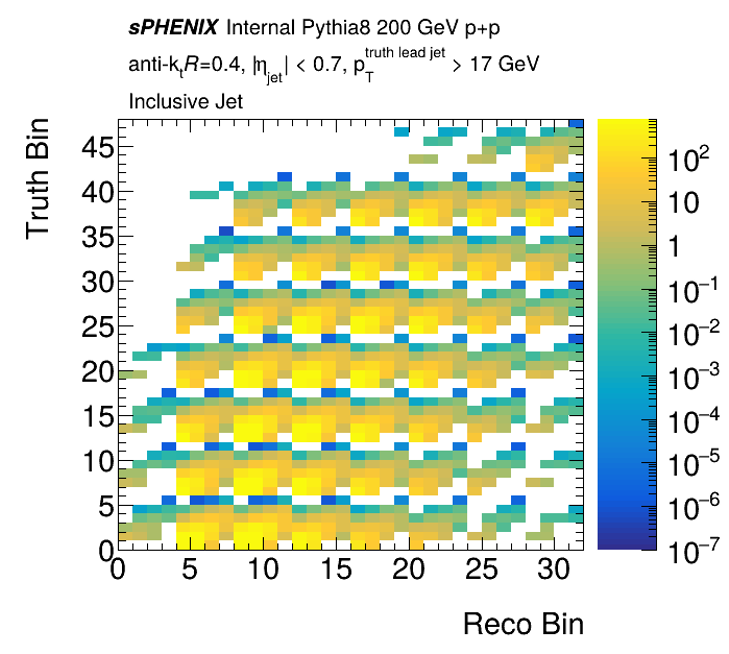
\includegraphics[width=0.48\linewidth]{Figures/unfolding/2D_response_matrix_inclusive.png}
    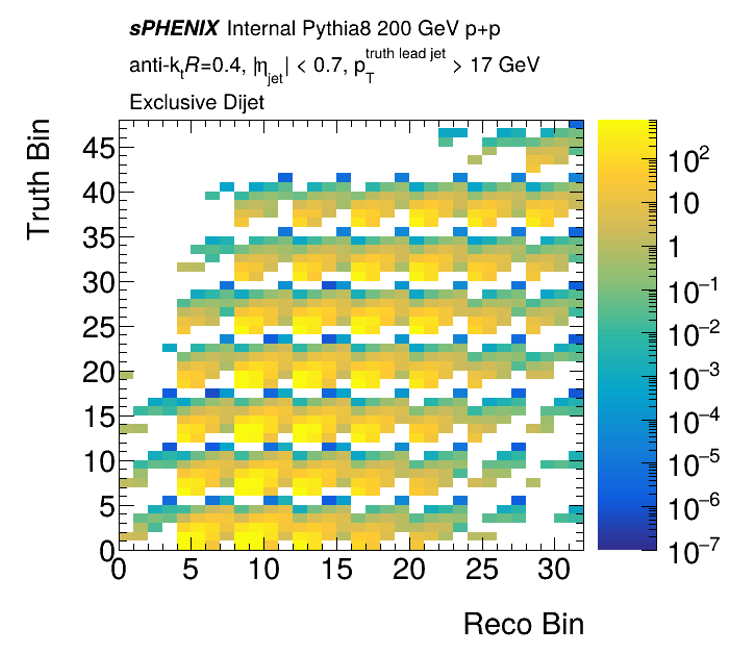
\includegraphics[width=0.48\linewidth]{Figures/unfolding/2D_response_matrix_dijet.png}
    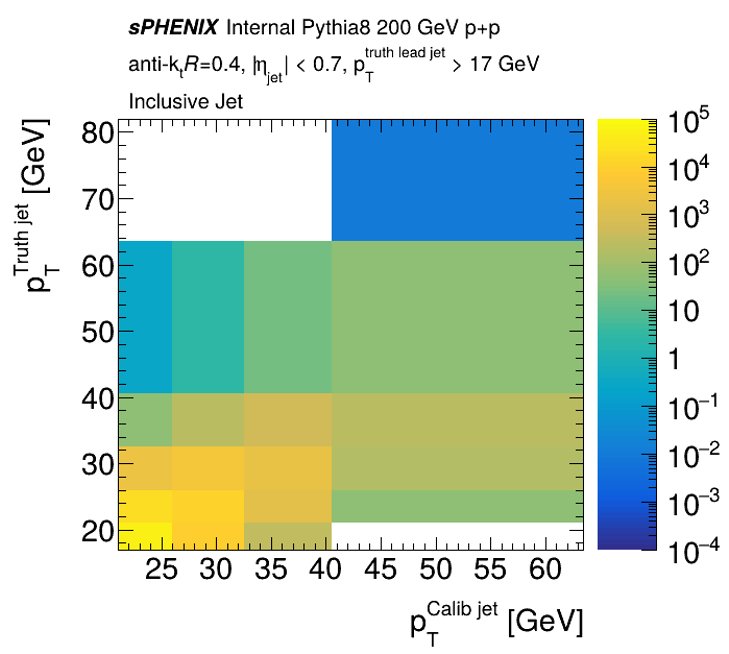
\includegraphics[width=0.48\linewidth]{Figures/unfolding/jetpt_response_matrix_inclusive.png}
    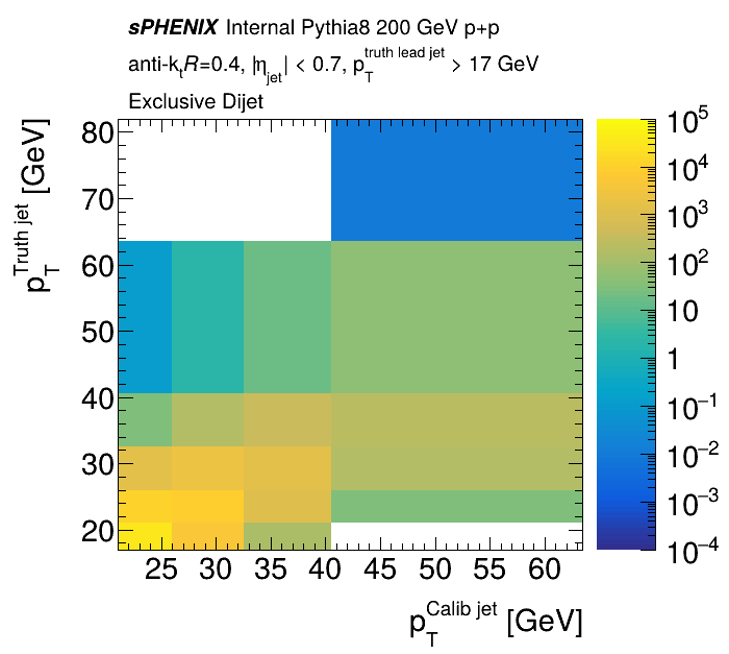
\includegraphics[width=0.48\linewidth]{Figures/unfolding/jetpt_response_matrix_dijet.png}
    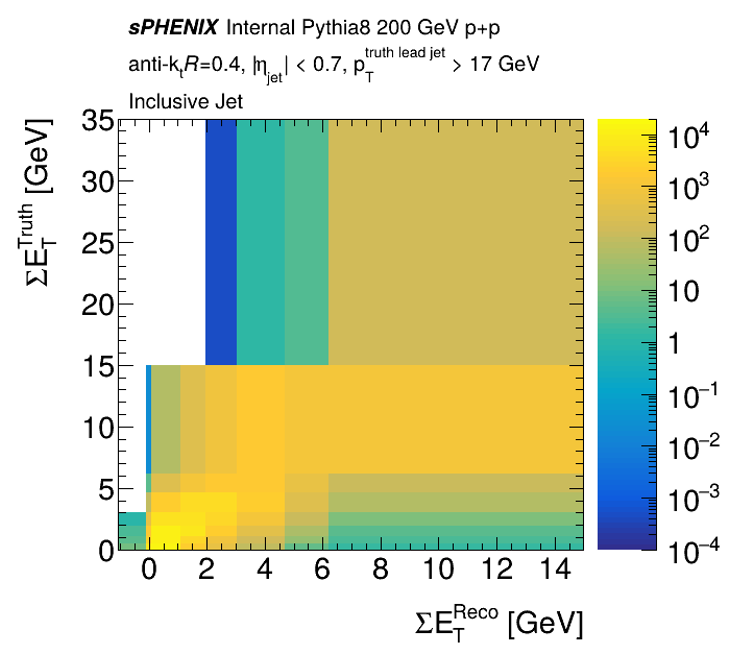
\includegraphics[width=0.48\linewidth]{Figures/unfolding/caloet_response_matrix_inclusive.png}
    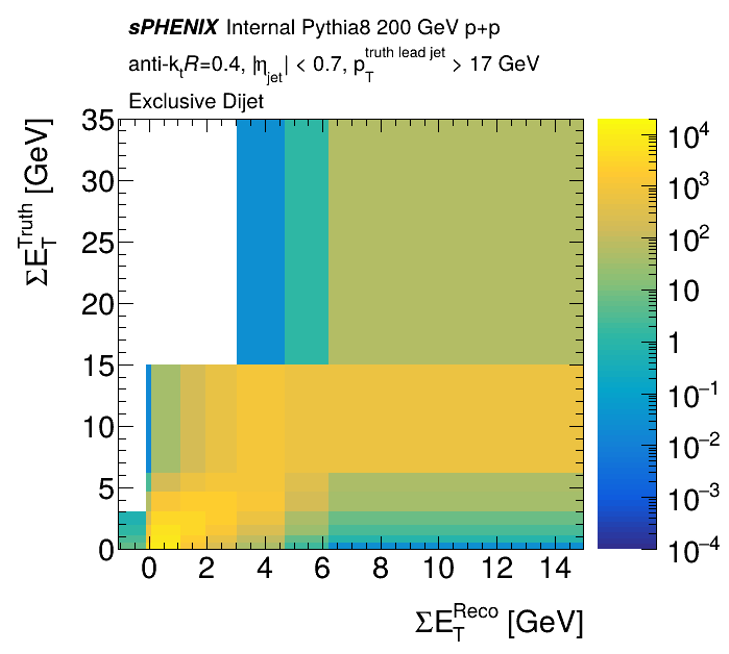
\includegraphics[width=0.48\linewidth]{Figures/unfolding/caloet_response_matrix_dijet.png}
    \caption{2D response matrix derived from simulation samples. The full 2D response matrix is shown with composite binning in the top plots for inclusive (left) and dijet (right) events. The 1D projections of this response matrix projected onto the leading jet $p_{T}$ (middle) and transverse region $\Sigma E_{T}$ (bottom) are also shown for inclusive (left) and dijet (right) events.}
    \label{fig:response_matrices}
\end{figure}

\subsubsection{MC Prior Reweighting for Unfolding}
To reduce prior dependence in the response, the simulation truth distributions are reweighted to match a data-driven pseudo-truth spectrum. 
The procedure uses the simulation response matrices and the data measured spectrum as inputs to a single-iteration RooUnfoldBayes pre-unfolding. 
For each response matrix variation (nominal and each systematic variation) and each trimming option (none, trim 5, trim 10), the unfolded pseudo-truth is normalized and divided by the normalized simulation truth to form a 2D weight matrix. 
These weights are applied to the original truth distribution to produce reweighted truth spectra that serve as priors for the subsequent response-matrix reweighting step. 

\begin{figure}
    \centering
    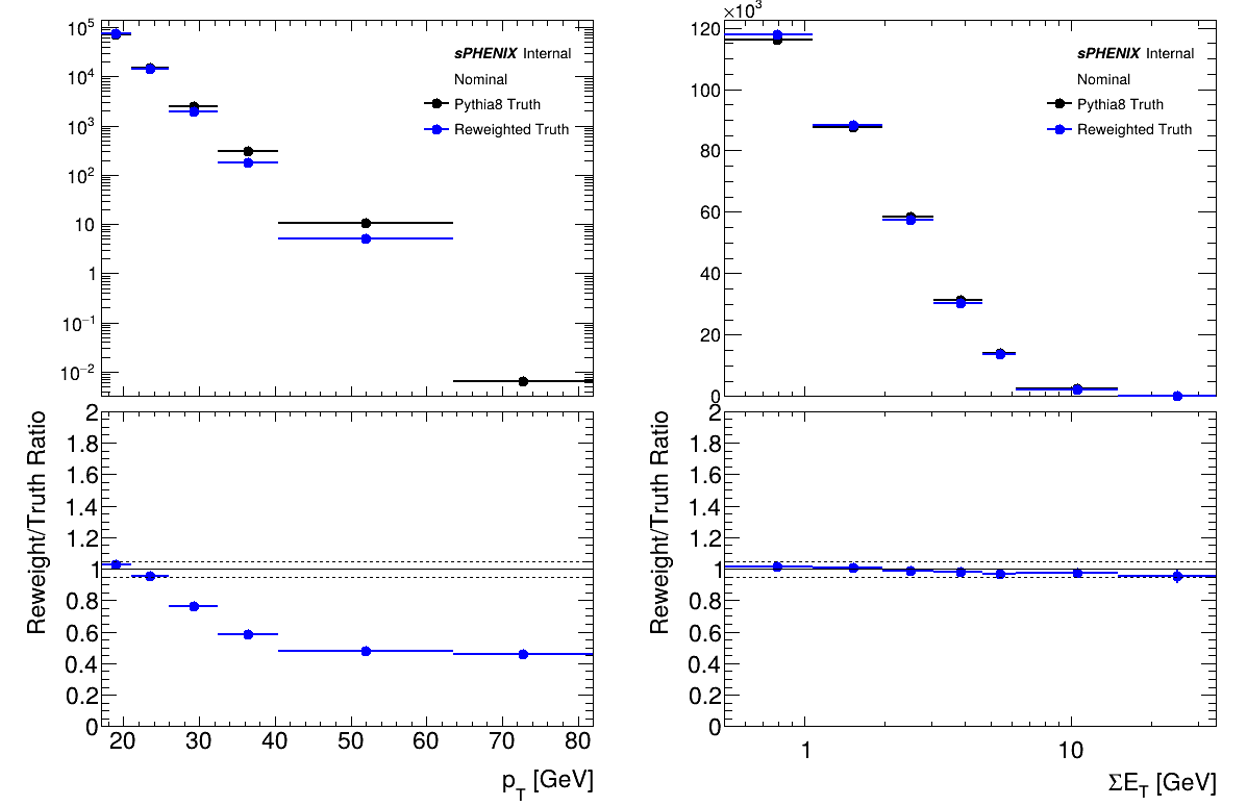
\includegraphics[height=0.4\textheight]{Figures/unfolding/prior_reweighting_inclusive.png}
    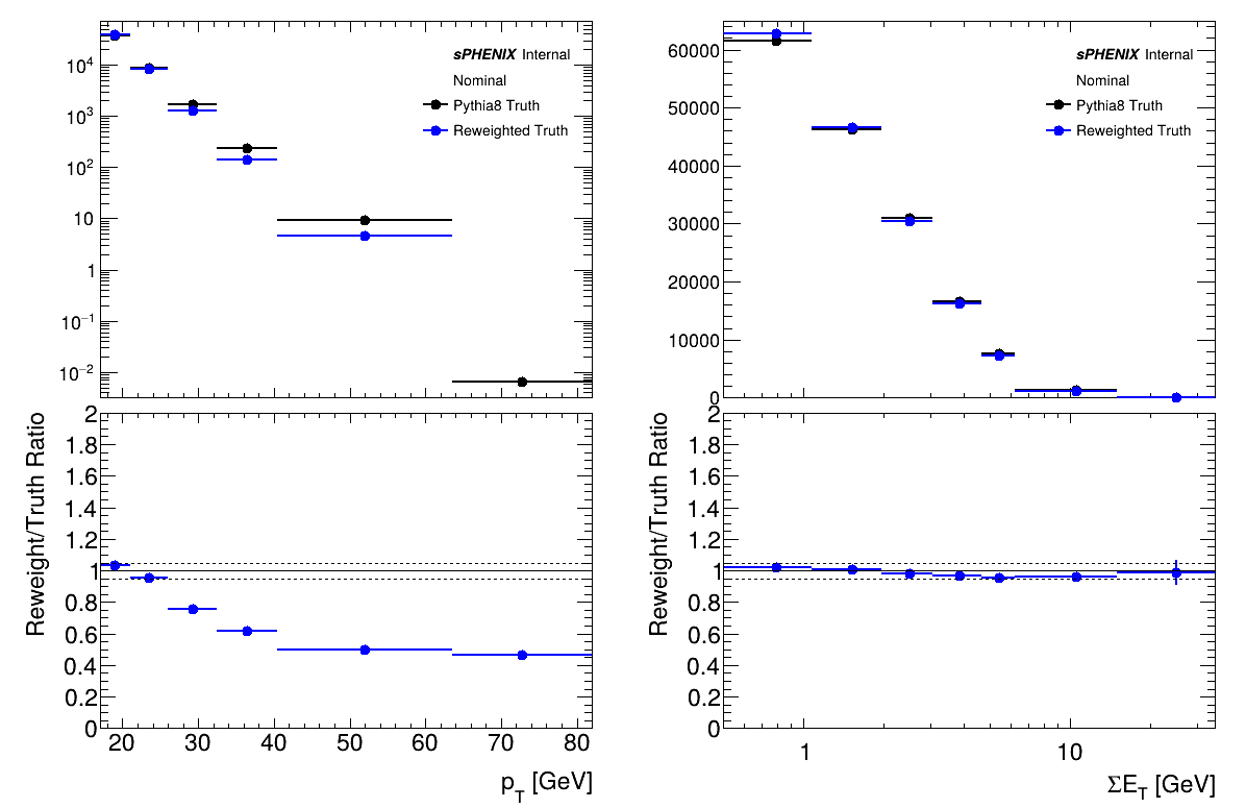
\includegraphics[height=0.4\textheight]{Figures/unfolding/prior_reweighting_dijet.png}
    \caption{Prior reweighting truth distributions for inclusive jet (top) and dijet (bottom) events. Projections onto the leading jet $p_{T}$ (left) and transverse region $\Sigma E_{T}$ (right) distribution axes before and after the full 2D prior reweighting for the nominal response matrix are shown.}
    \label{fig:prior_reweighting_truth}
\end{figure}

\subsubsection{Data Processing for Unfolding Procedure} 
The data processing module applies the unfolding selections as the simulation processing and event selections outlined in Section~\ref{sec:selection} to construct reconstructed level 2D histograms of $(p_{T}, \Sigma E_{T})$ spectra that are later unfolded.
Events are required to fire the jet 10 trigger (GL1 scaled trigger vector contains ID 22) and to pass the $z$-vertex selection ($|z_{\mathrm{vtx}}|<60$ cm). 
Reconstructed jets are filtered requiring $|\eta|<0.7$, positive jet energy, and eta within calorimeter acceptance, then the event must satisfy the minimum good jet multiplicity for jets passing acceptance filters and with $p_{T} > 2$ GeV (1 for inclusive, 2 for dijet). 
For dijets, the leading and subleading jets must pass the same energy ratio and azimuthal separation cuts as in simulation. 
For inclusive jet events, the leading-jet must pass the same energy-fraction cut as in simulation. 
Additionally, events with $\ge 9$ reconstructed jets above 5~GeV are rejected as bad events.

Timing cuts are applied using the reconstructed jet time and MBD timing: the leading jet time must lie within $[-8,4]$~ns, and a $\Delta t$ cut is applied either between the leading and subleading jets of $[-3,3]$~ns (dijet) or between the leading jet and MBD $t_{0}$ of $[-5,1]$~ns (inclusive). 
The leading jet $p_{T}$ is then calibrated with the JES correction, and trigger efficiency, timing cut efficiency and run-depedendent pileup corrections are applied as scale factors on the events filling the histogram.
The calibrated leading-jet $p_{T}$ and transverse $\Sigma E_{T}$ are mapped into the uniformized binning and filled into the 2D measured spectra used for unfolding.

\begin{table}[t]
    \centering
    \small
    \begin{tabular}{ll}
        \hline
        Data Selection & Definition \\
        \hline
        Trigger requirement & GL1 scaled trigger vector contains ID 22 \\
        Vertex cut & $|z_{\mathrm{vtx}}|<60$ cm \\
        Jet acceptance & $|\eta|<0.7$, positive energy, calo-$\eta$ acceptance \\
        Minimum reconstructed jets & 1 (inclusive) or 2 (dijet) ($p_{T}\ge 2$ GeV) \\
        Dijet background cut & $E_{\mathrm{sub}}/E_{\mathrm{lead}}>0.3$, $\Delta\phi>\Delta\phi_{\mathrm{min}} = 3\pi / 4$ \\
        Inclusive jet background cut & EMCal(10-90\%)/IHCal(0-90\%)/OHCal(10-90\%) lead jet E-fraction cut \\
        N$_{jet}$ background cut & reject events with $\ge 9$ jets ($p_{T}\ge 5$ GeV) \\
        Timing cuts & lead time in $[-8,4]$ ns; $\Delta t$ in $[-3,3]$ ns (dijet) or $[-5,1]$ ns (inclusive) \\
        JES correction & apply JES correction function \\
        Trigger efficiency & apply turn-on efficiency scale and variations \\
        Timing efficiency & apply timing-cut efficiency scale factor \\
        Pileup correction & apply run-dependent pileup correction to $\Sigma E_{T}$ \\
        \hline
    \end{tabular}
    \caption{Key selections and corrections applied in the data processing module for unfolding inputs.}
    \label{tab:data_unfold_processing}
\end{table}

\subsubsection{Closure Tests}
Closure tests are performed with the same response matrices used in the unfolding. 
Both a full-closure test, where each response matrix is unfolded against its own measured distribution with one Bayesian iteration, and a half-closure test, where the response from one half-sample is used to unfold the measured distribution from the complementary half-sample across 1--6 iterations, are performed. 
All nominal, JES/JER variations, and half-sample response matrices are tested for closure for each trimming option (none, trim 5, trim 10, and their reweighted counterparts). 
Statistical uncertainties on the closure spectra are evaluated with 1000 toy variations of the response matrix and combined in quadrature with the unfolded errors. 
The full closure and half closure tests for the nominal response matrix are shown in Figures~\ref{fig:full_closure_test_dijet} and \ref{fig:half_closure_test_dijet}. Both closure tests show agreement between the truth spectra and unfolded spectra of unity within statistical uncertainties. 

\begin{figure}
    \centering
    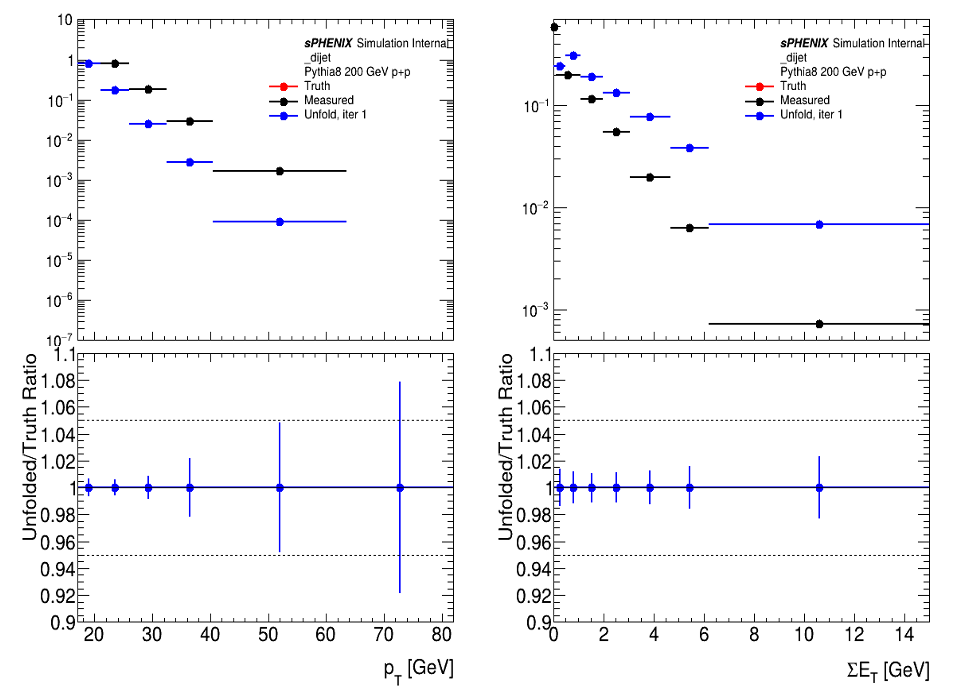
\includegraphics[height=0.45\textheight]{Figures/unfolding/dijet_full_closure.png}
    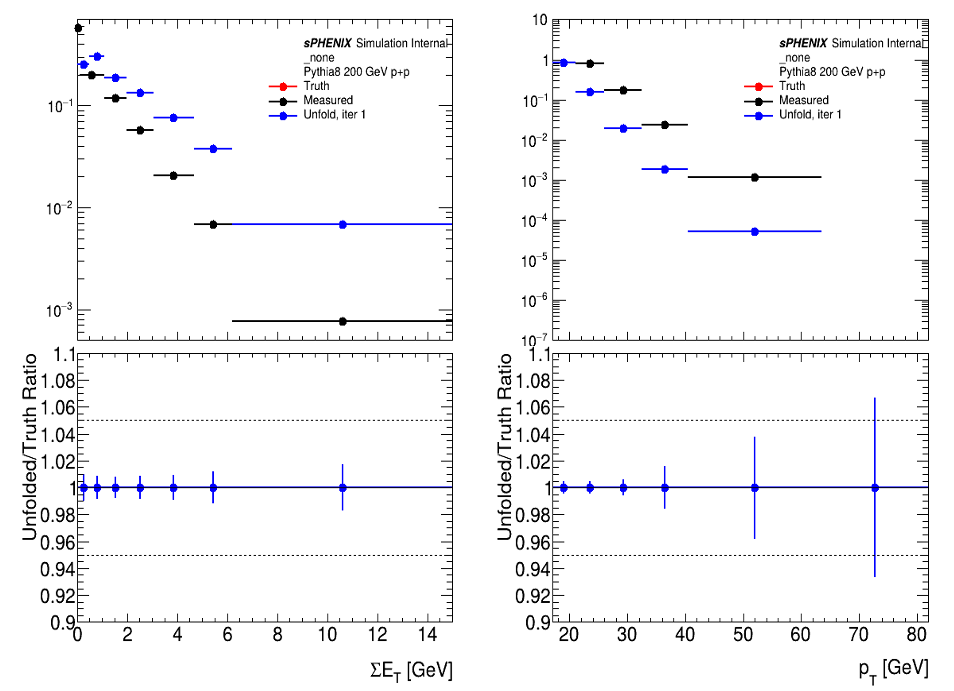
\includegraphics[height=0.45\textheight]{Figures/unfolding/inclusive_full_closure.png}
    \caption{Full-closure test results for dijet (top) and inclusive jet (bottom) events. The plots show both the truth, measured, and unfolded spectra for the reweighted and trimmed response matrices and below the unfolded-to-truth ratios for both jet $p_{T}$ (left) and transverse $\Sigma E_{T}$ (right).}
    \label{fig:full_closure_test_dijet}
\end{figure}

\begin{figure}
    \centering
    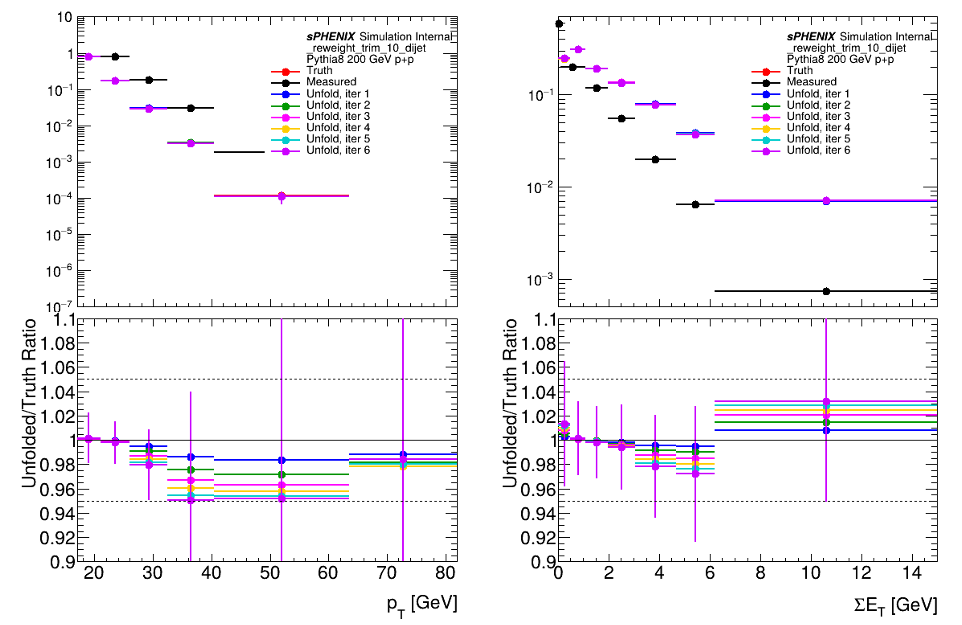
\includegraphics[height=0.45\textheight]{Figures/unfolding/dijet_half_closure.png}
    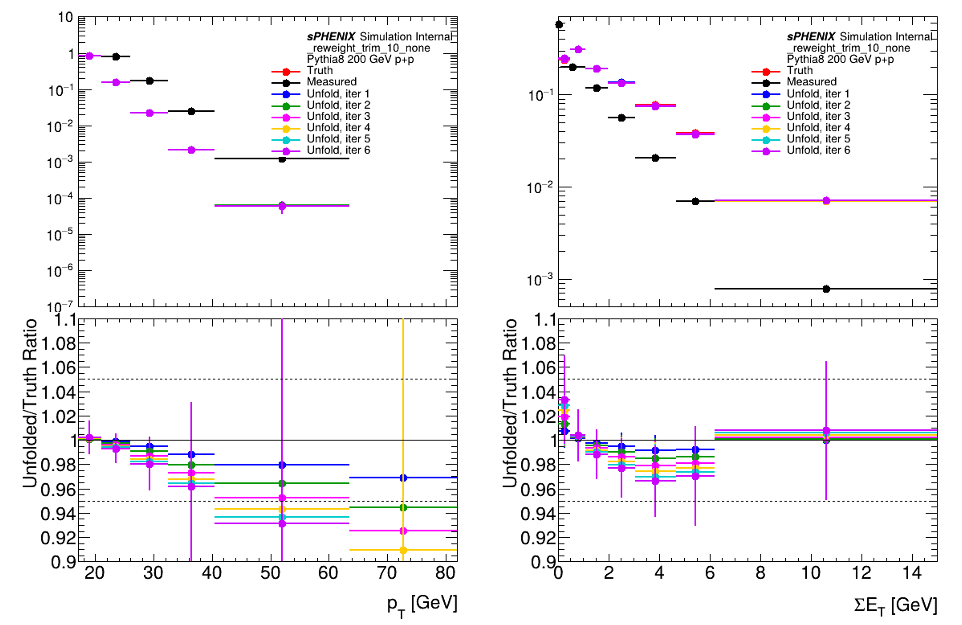
\includegraphics[height=0.45\textheight]{Figures/unfolding/inclusive_half_closure.png}
    \caption{Half-closure test results for dijet (top) and inclusive jet (bottom) events. The plots show both the truth, measured, and unfolded spectra for the reweighted and trimmed response matrices and below the unfolded-to-truth ratios for both jet $p_{T}$ (left) and transverse $\Sigma E_{T}$ (right).}
    \label{fig:half_closure_test_dijet}
\end{figure}

\subsubsection{Unfolding Data Results}
A 2D unfolding procedure in leading jet $p_{T}$ and transverse region $\Sigma E_{T}$ is performed using the response matrices derived from the three iteration simulation processing and the 2D histograms of reconstructed level information from data.
The unfolding is performed with the response matrices from simulation after both the trimming requirements and prior reweighting procedure for up to 20 iterations to determine a minimum in the unfolding process
where the change in unfolded result per iteration is at the level of the statistical precision of the measurement. 
Following this point in the iterative unfolding process the resulting statistical precision dominates the measurement result. 

Figure~\ref{fig:unfold_iterations} shows this iteration optimzation point for unfolding both inclusive jet and dijet event using the MC response matrix with a trimming requirement of 10 entries for each jet triggered MC sample and the prior reweighting procedure applied.
The two trends which define this minimum is the total change in unfolded values for each iteration in red and the total statistical error on the unfolded result in blue determined from the quadrature sum of the bin errors in the data histogram and the effect of statistical error in the response matrix tested by sampling 1000 toy models varying the response matrix bin values within 1$\sigma$ of their nominal value.
For both the inclusive jet and dijet results, the change in unfolded values per iteration x total statistical error curve has a minimum around 3 iterations, and thus 3 iterations is chosen as the optimal point for unfolding to balance minimizing prior dependence with minimizing statistical uncertainty in the measurement.
\begin{figure}
    \centering
    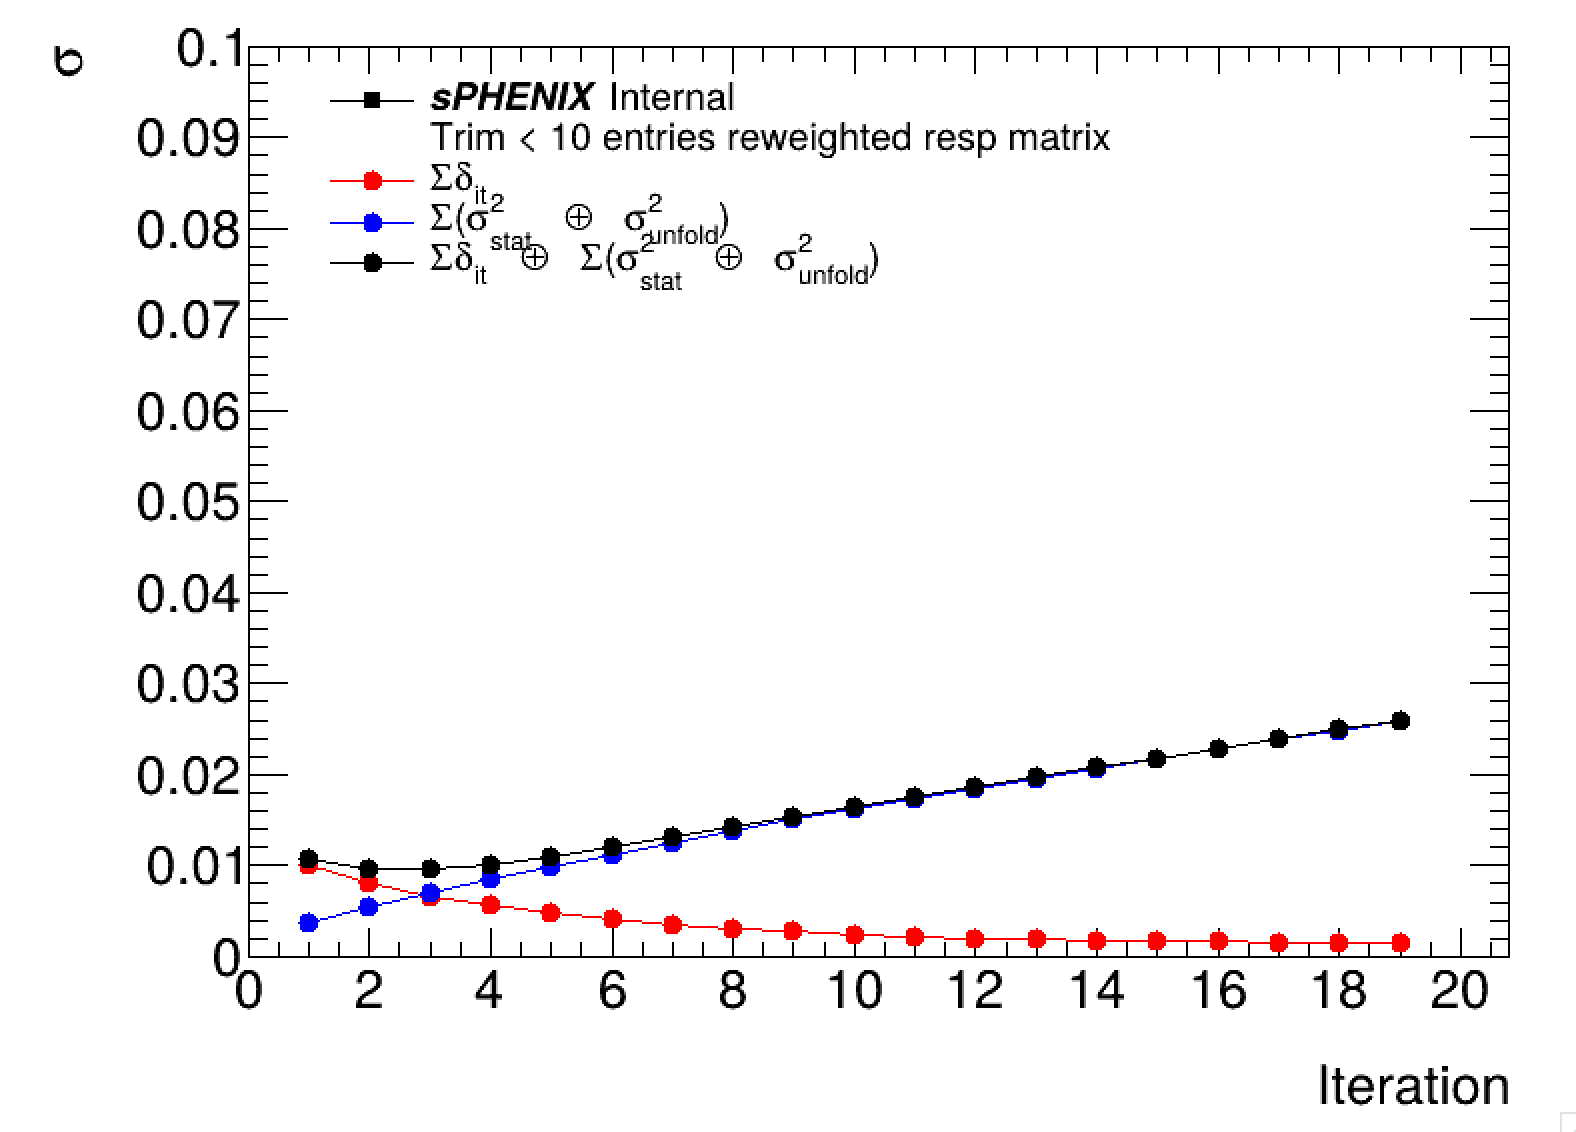
\includegraphics[width=0.48\linewidth]{Figures/unfolding/unfolding_iterations_inclusive.png}
    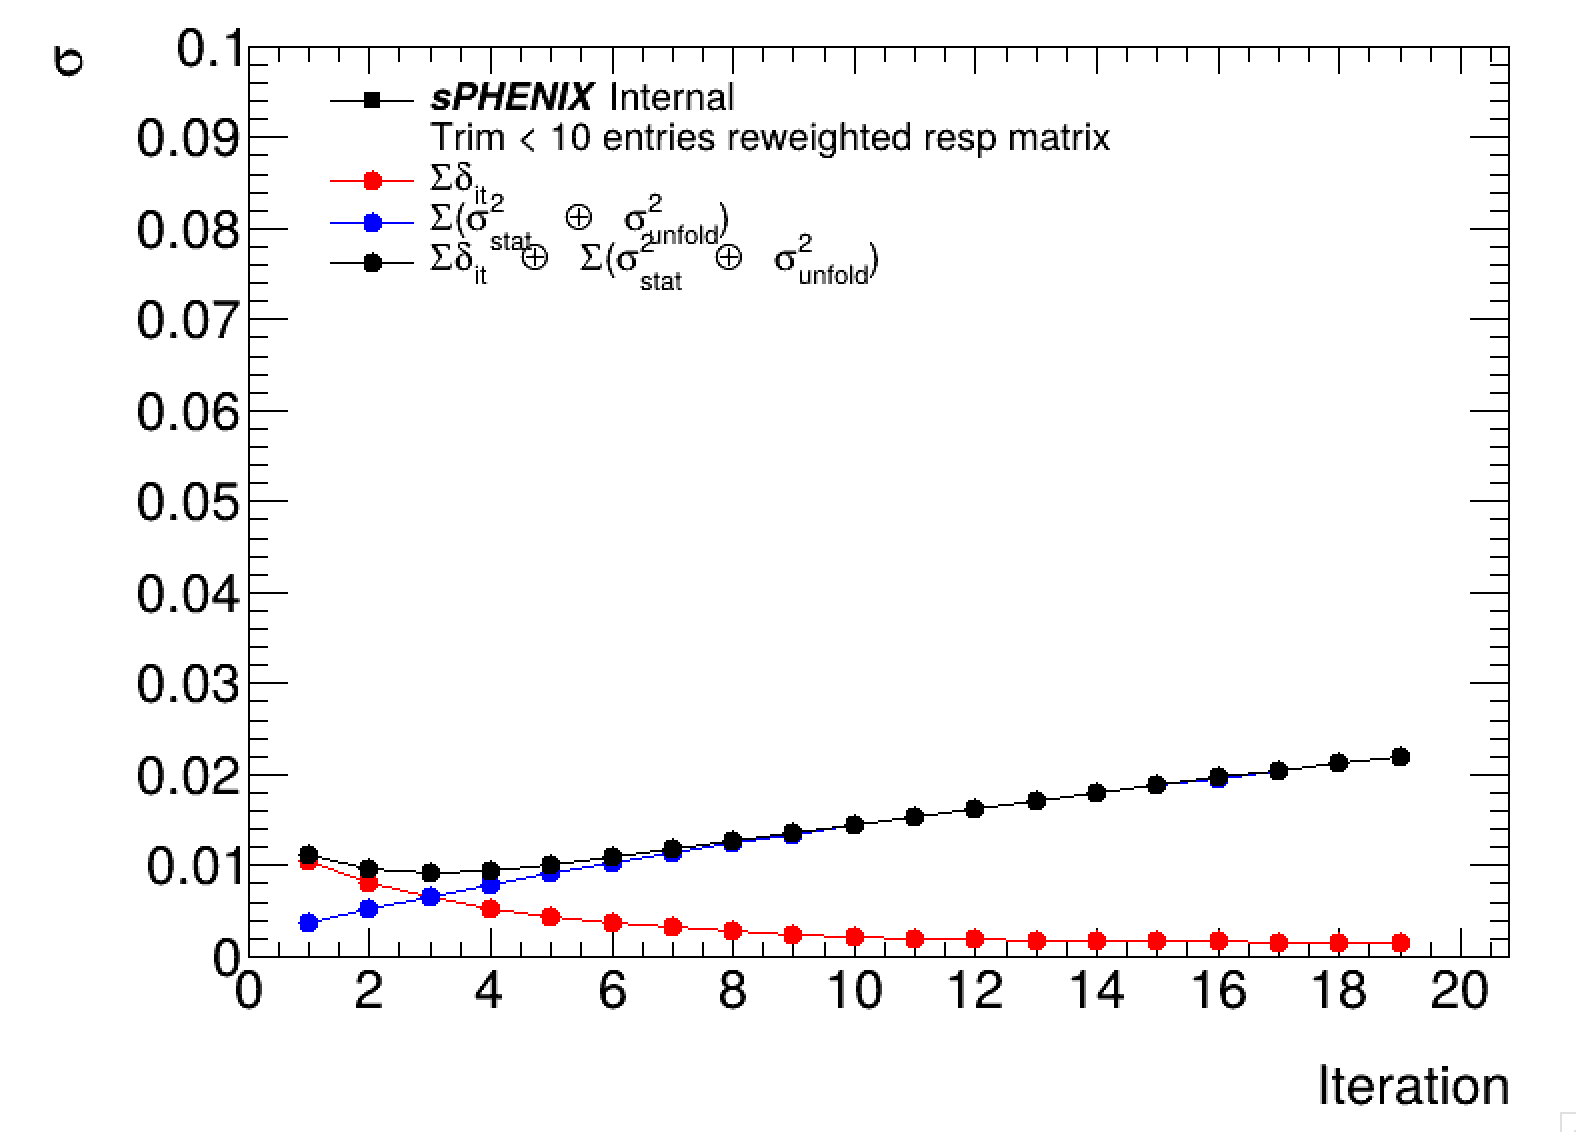
\includegraphics[width=0.48\linewidth]{Figures/unfolding/unfolding_iterations_dijet.png}
    \caption{Overall stability of unfolding procedure as a function of unfolding iterations for inclusive jet (left) and dijet (right) results. Total change in unfolded result per iteration shown red. Total statistical error in unfolded result per iteration shown in blue.}
    \label{fig:unfold_iterations}
\end{figure}

\subsection{Application of MBD Vertex Efficiency Correction}
\label{sec:mbd_vertex_eff_app}
The MBD vertex efficiency correction is applied as a scale factor to the unfolded $\Sigma E_{T}$ spectra to correct for the $\sim 5\%$ bias on the $\Sigma E_{T}$ spectra from the MBD-based vertex selection.
Figure~\ref{fig:mbd_vertex_eff_app} shows the effect of applying this efficinecy correction on the unfolded $\Sigma E_{T}$ spectra and unfolding average $\Sigma E_{T}$ as a function of leading jet $p_{T}$ for both inclusive jet and dijet events. 
There is a $1\%$ effect on the average $\Sigma E_{T}$ as a function of leading jet $p_{T}$, but a nearly uniform (on the order of 5\%) increase in the unfolded $\Sigma E_{T}$ spectra by approximately 1.4x for all $\Sigma E_{T}$ bins.

\begin{figure}
    \centering
    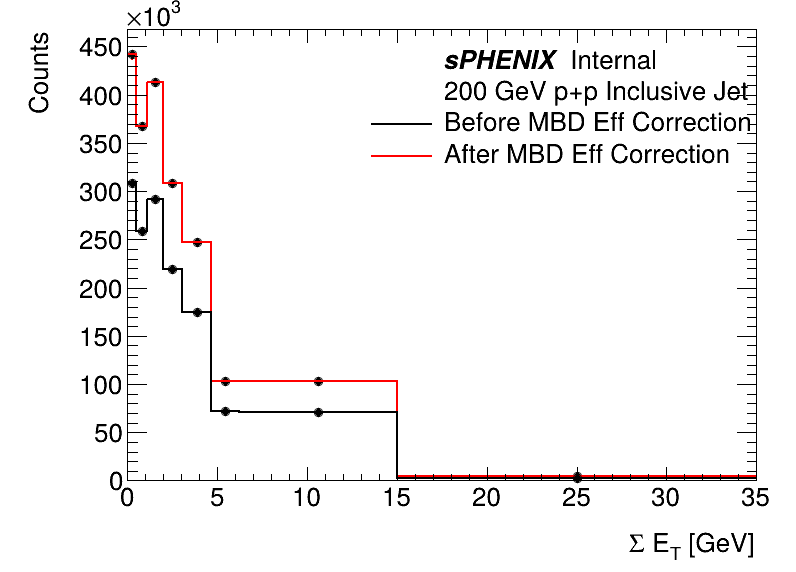
\includegraphics[width=0.48\linewidth]{Figures/mbd_vertex_efficiency/sphenix_primary_mbd_efficiency_effects_efrac_bkg_cut_projectionY.png}
    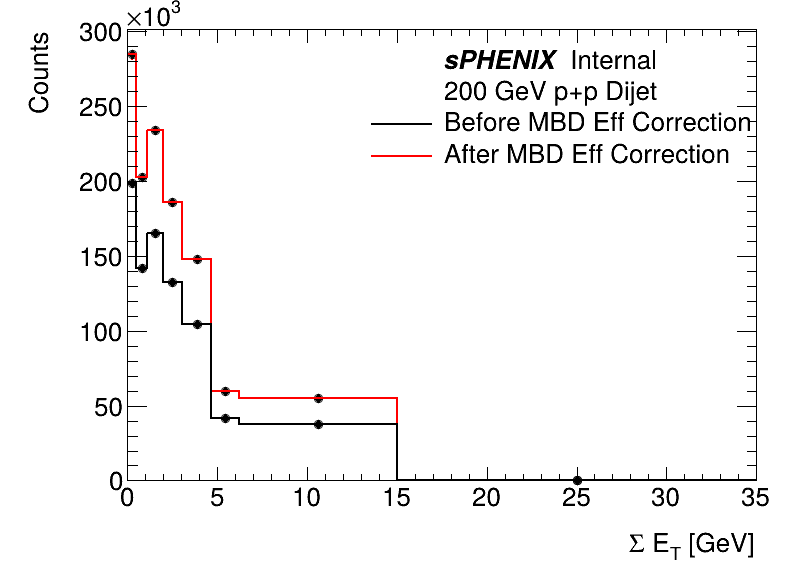
\includegraphics[width=0.48\linewidth]{Figures/mbd_vertex_efficiency/sphenix_primary_mbd_efficiency_effects_dijet_bkg_cut_projectionY.png}
    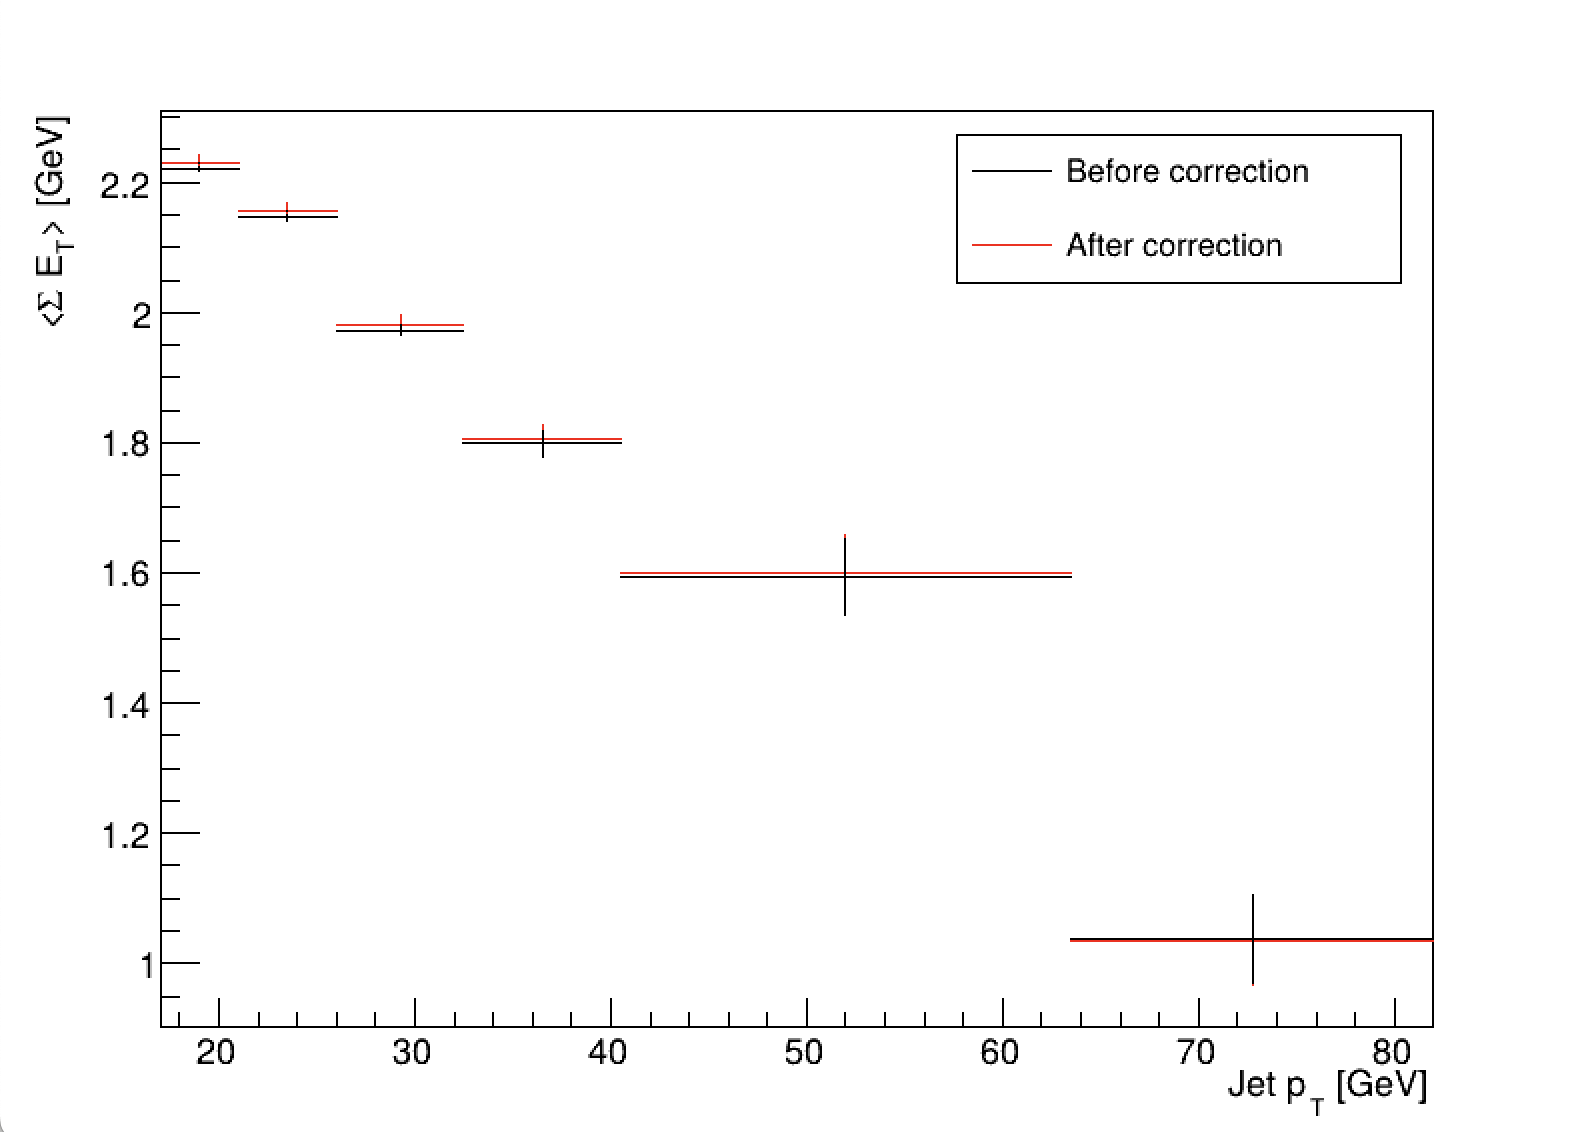
\includegraphics[width=0.48\linewidth]{Figures/mbd_vertex_efficiency/sphenix_primary_mbd_efficiency_effects_efrac_bkg_cut_profileX.png}
    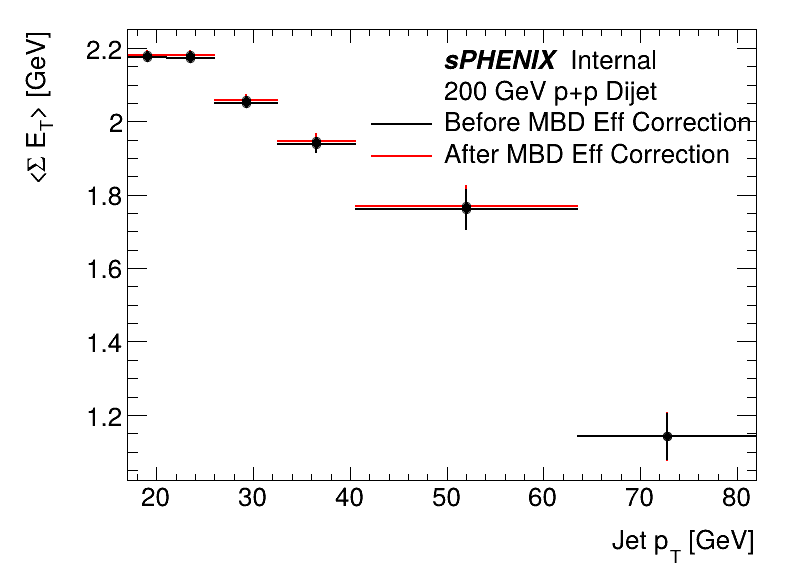
\includegraphics[width=0.48\linewidth]{Figures/mbd_vertex_efficiency/sphenix_primary_mbd_efficiency_effects_dijet_bkg_cut_profileX.png}
    \caption{Effect of applying MBD vertex efficiency correction on unfolded $\Sigma E_{T}$ spectra (top) and average $\Sigma E_{T}$ as a function of leading jet $p_{T}$ (bottom) for inclusive jet (left) and dijet (right) events.}
    \label{fig:mbd_vertex_eff_app}
\end{figure}
